\documentclass[aspectratio=169]{beamer}

% Theme — user-provided theme name per request
\usetheme{mybeamer}

% Placeholders you can change later
\newcommand{\RepoURL}{https://github.com/konradcinkusz/DeepDiveInto_CSharp_Dictionaries_presentation}
\newcommand{\BookURL}{https://github.com/konradcinkusz/BOOK_PLACEHOLDER}

% Title slide resources block (links colored to match the theme)
\titlegraphic{%
  \begingroup
    \footnotesize
    \faGithub\ \href{\RepoURL}{\textcolor{mbSecondary}{Presentation \& code (GitHub)}}%
    \quad\textbullet\quad
    \href{\BookURL}{\textcolor{mbSecondary}{Book draft “Deep Dive Into” — collaborate via PRs}}%
  \endgroup
}

% --- Packages ---
\usepackage[utf8]{inputenc}
\usepackage[T1]{fontenc}
\usepackage{lmodern}
\usepackage{microtype}
\usepackage{amsmath,amssymb}
\usepackage{booktabs}
\usepackage{array}
\usepackage{tikz}
\usetikzlibrary{arrows.meta,positioning,fit,calc,shapes.misc}

\newcolumntype{Y}{>{\raggedright\arraybackslash}X} % ragged-right, wrappable text
\newcolumntype{C}{>{\centering\arraybackslash}m{1.9cm}} % centered, fixed-width cell

% --- Meta (put in your preamble) ---
\title[Deep Dive: Dictionary<TKey,TValue>]{Deep Dive Into \texttt{Dictionary\textless TKey, TValue\textgreater} (C\#)}
\subtitle{From Ancient Times to Current State}
\author[\href{https://github.com/konradcinkusz}{dev\_insight \,|\, github.com/konradcinkusz}]{Konrad Cinkusz (\texttt{dev\_insight})}
\institute{C\# Collections Series}
\date{\today}

% Make footer link readable on the dark footline
\hypersetup{colorlinks=true, urlcolor=white}

% --- Helpers ---
\newcommand{\bigO}[1]{$\mathcal{O}(#1)$}
\newcommand{\code}[1]{\texttt{#1}}

% --- Document ---
\begin{document}

\begin{frame}
  \titlepage
\end{frame}

% ========================= Agenda / What We'll Do ============================
\begin{frame}{What We’re Going To Do}
  \begin{itemize}
    \item Establish the \textbf{problem}: fast key $\rightarrow$ value lookup at scale.
    \item Follow a \textbf{timeline} using one conceptual dataset throughout:
      \begin{itemize}
        \item \textbf{Ancient times}: linear search \& \code{Hashtable} (pre-generics).
        \item \textbf{Middle ages}: \code{Dictionary<TKey,TValue>} (generics, hashing done right).
        \item \textbf{Current times}: specialized maps for real-world needs
              (\code{ConcurrentDictionary}, \code{ImmutableDictionary}, \code{FrozenDictionary}).
      \end{itemize}
    \item Peek into \textbf{internals}: buckets, entries, hashing, collisions, resizing.
    \item Discuss \textbf{testing/benchmarking} for complexity evidence (no code, methodology only).
    \item Close with \textbf{best practices}, pitfalls, and a \textbf{decision matrix}.
  \end{itemize}
\end{frame}

% ========================= Shared Dataset (Conceptual) =======================
\begin{frame}{Shared Dataset (Conceptual)}
  \textbf{Single dataset used across all eras:}
  \begin{itemize}
    \item \textbf{Key}: \code{ProductId} $\rightarrow$ pair \code{(Category:string, Number:int)}.
    \item \textbf{Value}: \code{Product} $\rightarrow$ \code{(Id:ProductId, Name:string, Price:decimal)}.
  \end{itemize}
  \textbf{Key properties we rely on:}
  \begin{itemize}
    \item \textbf{Immutability} (conceptually): key state does not change after insertion.
    \item \textbf{Stable equality \& hash}: consistent \code{Equals} \& \code{GetHashCode}.
    \item \textbf{Comparer choice matters}: e.g., ordinal vs culture-aware, case-sensitive vs insensitive.
  \end{itemize}
  \textbf{Why the same dataset?} Ensures apples-to-apples comparisons between eras and structures.
\end{frame}

% ========================= Why Dictionaries Exist ===========================
\begin{frame}{Why Do We Have Dictionaries?}
  \begin{itemize}
    \item \textbf{Goal}: sublinear or constant-time lookup independent of collection size.
    \item \textbf{Linear search} across arrays/lists is \bigO{n} per query.
    \item \textbf{Hash tables} target \bigO{1} average-time operations (Add/Remove/Lookup), given:
      \begin{itemize}
        \item Good hash distribution (\emph{few collisions}).
        \item Appropriate \textbf{capacity} and load factor.
        \item \textbf{Stable keys} (hash value doesn’t change while stored).
      \end{itemize}
    \item Dictionaries are the \textbf{generic}, \textbf{type-safe}, high-level hash table in .NET.
  \end{itemize}
\end{frame}

% ========================= Complexity Overview ==============================
\begin{frame}{Complexity Overview}
  \begin{columns}[T,onlytextwidth]
    \column{0.60\textwidth}
    \begin{block}{Time Complexity (Typical)}
      \small
      \setlength{\tabcolsep}{4pt}
      \renewcommand{\arraystretch}{1.1}
      \begin{tabularx}{\linewidth}{@{}l
          >{\centering\arraybackslash}m{1.9cm}
          >{\centering\arraybackslash}m{1.9cm}@{}}
        \toprule
        \textbf{Structure} & \textbf{Average} & \textbf{Worst} \\
        \midrule
        Linear search (array/list) & \bigO{n} & \bigO{n} \\
        \code{Hashtable}           & \bigO{1} & \bigO{n} \\
        \code{Dictionary}          & \bigO{1} & \bigO{n} \\
        \code{SortedDictionary}    & \bigO{\log n} & \bigO{\log n} \\
        \code{ConcurrentDictionary}& \bigO{1} & \bigO{n} \\
        \code{ImmutableDictionary} & \bigO{1}\,\footnotesize(avg) & \bigO{n} \\
        \code{FrozenDictionary}    & \bigO{1}\,\footnotesize(read) & \bigO{n} \\
        \bottomrule
      \end{tabularx}
      \vspace{0.3em}
      \footnotesize\textit{Notes: Immutable — average-case lookup; Frozen — read-only lookups.}
    \end{block}

    \column{0.40\textwidth}
    \begin{block}{Space Complexity}
      \small
      \begin{itemize}
        \setlength\itemsep{2pt}
        \item Dictionaries: \bigO{n} entries plus overhead for buckets/entries.
        \item Overhead depends on load factor and collision chains.
        \item \textbf{Frozen} trades build-time memory for faster reads and compact layout.
      \end{itemize}
    \end{block}
  \end{columns}
\end{frame}

% ========================= Internals Diagram (fixed) ==========================
\begin{frame}{Dictionary Internals (Conceptual Diagram)}
  \centering
  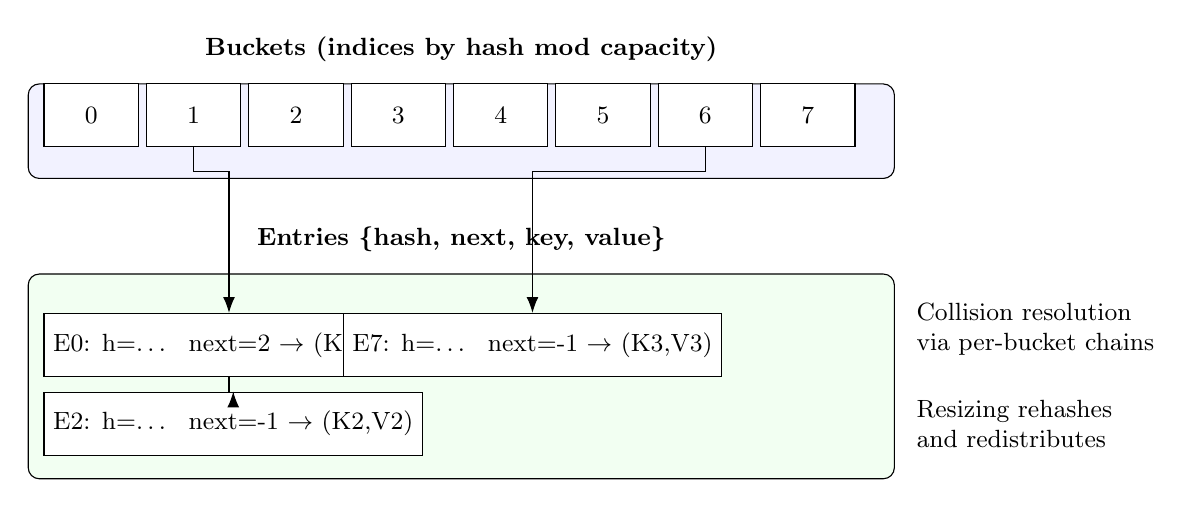
\begin{tikzpicture}[font=\small, node distance=6mm]
    % Buckets container box
    \node[draw, rounded corners, minimum width=11cm, minimum height=1.2cm, fill=blue!5] (BucketsBox) {};
    % Title above buckets
    \node[anchor=south] at ($(BucketsBox.north)+(0,0.15cm)$) {\textbf{Buckets (indices by hash mod capacity)}};

    % Individual bucket cells
    \foreach \i in {0,...,7} {
      \node[
        draw, fill=white,
        minimum width=1.2cm, minimum height=0.8cm,
        anchor=west
      ] (buck\i) at ($(BucketsBox.west)+(0.2cm,0.2cm) + \i*(1.3cm,0)$) {\i};
    }

    % Entries container box
    \node[draw, rounded corners, minimum width=11cm, minimum height=2.6cm, fill=green!5, below=1.2cm of BucketsBox] (EntriesBox) {};
    % Title above entries
    \node[anchor=south] at ($(EntriesBox.north)+(0,0.15cm)$) {\textbf{Entries \{hash, next, key, value\}}};

    % Some fake entries
    \node[draw, fill=white, minimum height=0.8cm, minimum width=3.6cm, anchor=west]
      (e1) at ($(EntriesBox.west)+(0.2cm,0.4cm)$) {E0: h=\dots\; next=2 $\rightarrow$ (K1,V1)};
    \node[draw, fill=white, minimum height=0.8cm, minimum width=3.6cm, anchor=west]
      (e2) at ($(EntriesBox.west)+(0.2cm,-0.6cm)$) {E2: h=\dots\; next=-1 $\rightarrow$ (K2,V2)};
    \node[draw, fill=white, minimum height=0.8cm, minimum width=3.6cm, anchor=west]
      (e3) at ($(EntriesBox.west)+(4.0cm,0.4cm)$) {E7: h=\dots\; next=-1 $\rightarrow$ (K3,V3)};

    % Arrows from buckets to entries (collision chains)
    \draw[-{Latex[length=2mm]}] (buck1.south) -- ++(0,-0.3) -| (e1.north);
    \draw[-{Latex[length=2mm]}] (e1.south) -- ++(0,-0.2) -| (e2.north);
    \draw[-{Latex[length=2mm]}] (buck6.south) -- ++(0,-0.3) -| (e3.north);

    % Notes at the side
    \node[align=left, anchor=west] at ($(EntriesBox.east)+(0.15cm,0.6cm)$) {Collision resolution\\via per-bucket chains};
    \node[align=left, anchor=west] at ($(EntriesBox.east)+(0.15cm,-0.6cm)$) {Resizing rehashes\\and redistributes};
  \end{tikzpicture}

  \vspace{1ex}
  \footnotesize
  \textit{Conceptual view: hash $\Rightarrow$ bucket index; bucket points to first entry; collisions follow \code{next} links.}
\end{frame}


% ========================= Testing / Benchmarks ==============================
\begin{frame}{Testing \& Benchmarks (Methodology)}
  \textbf{Purpose}: illustrate the shape of growth and relative costs (not exact nanoseconds).
  \begin{itemize}
    \item \textbf{Scenarios}
      \begin{itemize}
        \item Lookup \textbf{hit vs miss} for: \code{Dictionary}, \code{Hashtable}, \code{SortedDictionary}, \code{Concurrent}, \code{Immutable}, \code{Frozen}.
        \item \textbf{Exception path} (indexer miss throwing) vs \code{TryGetValue}.
        \item \textbf{Capacity} effects: default vs pre-sized build, allocations.
        \item \textbf{Pathological collisions}: poor hash distribution.
      \end{itemize}
    \item \textbf{Controls}
      \begin{itemize}
        \item Same dataset across contenders; release build; no debugger.
        \item Repeat runs; measure time and allocations.
      \end{itemize}
    \item \textbf{Interpretation}
      \begin{itemize}
        \item Focus on \textbf{trends}: flat \bigO{1} vs growing \bigO{n}/\bigO{\log n}.
        \item Avoid overfitting tiny differences; highlight orders of magnitude.
      \end{itemize}
  \end{itemize}
\end{frame}

% ========================= Ancient Times =====================================
\begin{frame}{Ancient Times: Linear Search \& \code{Hashtable}}
  \begin{itemize}
    \item \textbf{Linear search} (\bigO{n}) over arrays/lists: simple but scales poorly.
    \item \code{Hashtable} (pre-generics):
      \begin{itemize}
        \item Keys/values are \code{object} $\Rightarrow$ \textbf{boxing} for value-type keys, \textbf{casts} on read.
        \item \textbf{Type safety pitfalls}: mixed types compile, fail at runtime.
        \item Lookup semantics: missing key typically returns \code{null} (subtle bugs if unchecked).
      \end{itemize}
    \item Lessons:
      \begin{itemize}
        \item Non-generic containers cost correctness and performance.
        \item We want type safety + fast lookups $\Rightarrow$ generics \& \code{Dictionary}.
      \end{itemize}
  \end{itemize}
\end{frame}

% ========================= Middle Ages =======================================
\begin{frame}{Middle Ages: \code{Dictionary<TKey,TValue>} Arrives}
  \begin{itemize}
    \item \textbf{Type-safe}, \textbf{generic} hash table: no boxing for struct keys, no casts on read.
    \item Core operations: \code{Add}, indexer (\emph{throws if missing}), \code{TryGetValue}, \code{TryAdd}, \code{Remove}.
    \item \textbf{Comparers}: pass \code{IEqualityComparer<TKey>} to define equality (e.g., case-insensitive).
    \item \textbf{Capacity planning}: constructor capacity; \code{EnsureCapacity}; \code{TrimExcess}.
    \item \textbf{Iteration}: \bigO{n}; order reflects internal organization (not a sorting guarantee).
  \end{itemize}
\end{frame}

\begin{frame}{Dictionary: Correctness Requirements}
  \begin{itemize}
    \item \textbf{Immutable keys}: do not mutate fields that affect \code{GetHashCode}/\code{Equals} after insertion.
    \item \textbf{Stable hashing}: equal keys must produce equal hashes; hash must remain stable while stored.
    \item \textbf{Good distribution}: avoid clustered hashes to reduce collision chains.
    \item \textbf{Comparer alignment}: ensure equality semantics match the domain (ordinal vs culture-aware).
  \end{itemize}
\end{frame}

\begin{frame}{Dictionary: Performance Factors}
  \begin{itemize}
    \item \textbf{Load factor \& capacity}: fewer resizes $\Rightarrow$ fewer rehashes $\Rightarrow$ fewer cache misses.
    \item \textbf{Collisions}: per-bucket chains increase probe length; worst case degrades to \bigO{n}.
    \item \textbf{Exceptions are expensive}: prefer \code{TryGetValue} over indexer misses in hot paths.
    \item \textbf{Allocation behavior}: entries and buckets arrays; resizing grows capacity geometrically.
  \end{itemize}
\end{frame}

% ========================= Current Times =====================================
\begin{frame}{Current Times: Choosing Specialized Maps}
  \begin{itemize}
    \item \code{ConcurrentDictionary<TKey,TValue>}
      \begin{itemize}
        \item Thread-safe reads/writes without external locking.
        \item Atomic operations: \code{GetOrAdd}, \code{AddOrUpdate}.
        \item Overhead vs single-threaded \code{Dictionary}.
      \end{itemize}
    \item \code{ImmutableDictionary<TKey,TValue>}
      \begin{itemize}
        \item \textbf{Persistent} structure: updates create new versions (structural sharing).
        \item Ideal for many readers, few writers; thread-safe reads by design.
      \end{itemize}
    \item \code{FrozenDictionary<TKey,TValue>}
      \begin{itemize}
        \item Build once; optimized layout for \textbf{very fast lookups}.
        \item Great for hot, read-only tables (configuration, token maps).
      \end{itemize}
  \end{itemize}
\end{frame}

% ========================= Decision Matrix ===================================
\begin{frame}{Decision Matrix}
  \small
  \setlength{\tabcolsep}{4pt}       % tighter horizontal padding
  \renewcommand{\arraystretch}{1.15}% comfortable row height
  \centering
  \begin{tabularx}{\linewidth}{@{}Y >{\ttfamily\footnotesize\arraybackslash}m{4.9cm} C@{}}
    \toprule
    \textbf{Need} & \textbf{Pick} & \textbf{Lookup} \\
    \midrule
    Single-threaded, mutable, fastest average-time
      & \texttt{Dictionary\textless TKey,\,TValue\textgreater}
      & \bigO{1} avg \\
    Many concurrent writers
      & \texttt{ConcurrentDictionary\textless TKey,\,TValue\textgreater}
      & \bigO{1} avg \\
    Many readers, safe sharing, versioned updates
      & \texttt{ImmutableDictionary\textless TKey,\,TValue\textgreater}
      & \bigO{1} avg \\
    Build once, read a lot (hot path)
      & \texttt{FrozenDictionary\textless TKey,\,TValue\textgreater}
      & \bigO{1} read \\
    Sorted order by key
      & \texttt{SortedDictionary\textless TKey,\,TValue\textgreater}
      & \bigO{\log n} \\
    Preserve insertion order (non-generic)
      & \texttt{OrderedDictionary}
      & \bigO{1} avg \\
    \bottomrule
  \end{tabularx}
\end{frame}

% ========================= Pitfalls & Best Practices =========================
\begin{frame}{Pitfalls \& Best Practices}
  \begin{columns}[T,onlytextwidth]
    \column{0.52\textwidth}
    \textbf{Pitfalls}
    \begin{itemize}
      \item \textbf{Mutable keys}: changing key fields after insertion breaks lookup/removal.
      \item \textbf{Poor hashes}: collisions inflate probe chains $\Rightarrow$ \bigO{n}.
      \item \textbf{Exceptions as control flow}: indexer miss throws; costly in hot paths.
      \item \textbf{Modifying during enumeration}: invalidates enumerator.
      \item \textbf{Wrong comparer}: culture-sensitive equality when ordinal needed (or vice versa).
    \end{itemize}
    \column{0.48\textwidth}
    \textbf{Best Practices}
    \begin{itemize}
      \item Use \textbf{immutable keys} (records/readonly structs, strings, GUIDs).
      \item Prefer \code{TryGetValue}/\code{TryAdd} in hot paths.
      \item \textbf{Pre-size} via constructor or \code{EnsureCapacity}.
      \item Choose the \textbf{right comparer} for semantics and performance.
      \item Pick the \textbf{right map} for concurrency/immutability/ordering needs.
    \end{itemize}
  \end{columns}
\end{frame}

% ========================= Testing: What to Show =============================
\begin{frame}{Testing: What to Show (No Code, Just Results)}
  \begin{itemize}
    \item \textbf{Lookup hit vs miss} across structures (flat vs growing curves).
    \item \textbf{Indexer miss exception} vs \code{TryGetValue(false)} (orders-of-magnitude difference).
    \item \textbf{Capacity planning}: default vs pre-sized build time and allocations.
    \item \textbf{Collision worst case}: deliberately bad hash to visualize degradation.
    \item Present with:
      \begin{itemize}
        \item Tables for mean time \& allocations.
        \item Line charts: time vs $n$ for linear search, sorted, and dictionary (flat).
      \end{itemize}
  \end{itemize}
\end{frame}

% ========================= Culture & Comparers ===============================
\begin{frame}{Equality \& Comparers (Strings as Keys)}
  \begin{itemize}
    \item \textbf{Ordinal vs Culture-aware}: choose based on domain semantics (identifiers vs UI text).
    \item \textbf{Case sensitivity}: \code{OrdinalIgnoreCase} for case-insensitive identifiers.
    \item \textbf{Custom comparers}: implement \code{IEqualityComparer<TKey>} to define equality \& hash together.
    \item \textbf{Consistency}: equality and hash must agree (equal $\Rightarrow$ equal hash).
  \end{itemize}
\end{frame}

% ========================= Memory & Resizing =================================
\begin{frame}{Memory Layout \& Resizing (High Level)}
  \begin{itemize}
    \item \textbf{Buckets array} indexes into an \textbf{entries array}.
    \item Each entry stores \emph{hash}, \emph{next pointer/index}, \emph{key}, \emph{value}.
    \item \textbf{Load factor threshold} triggers resize:
      \begin{itemize}
        \item New capacity, rehash, redistribute entries.
        \item Costly operation; plan capacity to minimize frequency.
      \end{itemize}
    \item \textbf{Iteration} is \bigO{n}; order follows internal entry sequence (not a sorting guarantee).
  \end{itemize}
\end{frame}

% ========================= Summary ===========================================
\begin{frame}{Summary \& Takeaways}
  \begin{itemize}
    \item \textbf{Dictionaries} deliver \bigO{1} average-time lookups with the right keys and capacity.
    \item \textbf{Keys} must be immutable with stable equality \& hashing; pick the correct \textbf{comparer}.
    \item Prefer \code{TryGetValue} and \textbf{pre-size} when possible.
    \item For \textbf{concurrency/immutability}, consider \code{ConcurrentDictionary} / \code{ImmutableDictionary}.
    \item For hot \textbf{read-only} tables, \code{FrozenDictionary} can be ideal.
    \item Always validate with \textbf{benchmarks}; focus on trend lines, not tiny deltas.
  \end{itemize}
\end{frame}

% ========================= Thank You =========================================
\begin{frame}[standout]
  Thank you! \\
  \vspace{2mm}
  Questions?
\end{frame}

\end{document}
